\documentclass[11pt]{book}
\usepackage{amssymb,amsmath,epsfig,fancyhdr,enumerate, caption, pst-node,anysize}
\usepackage{float, graphics,amsfonts,latexsym,epstopdf, import}
\usepackage[utf8]{inputenc}
\usepackage[spanish]{babel}
\usepackage{amsthm} %% Para la definición de los teoremas



%% Para cambiar el tipo de letra
\usepackage[T1]{fontenc}
\usepackage{accanthis}
%%



%%%% Para imágenes
\usepackage{graphicx}
\graphicspath{ {images/} }
\usepackage{subcaption} % Para múltiples imágenes
\usepackage{caption} % Para el texto de las imágenes



%%%%% para los apéndices
\usepackage[toc,page]{appendix}


%%%% Estilo de la pagina
\pagestyle{fancyplain}
%%%Que la linea de la cabecera este del tamaño del texto de la cabecera
\addtolength{\headwidth}{-25pt}

\renewcommand{\sectionmark}[1]%
                 {\markright{\thesection\ #1}}

\newcommand{\clearemptypage}{ %
                \newpage{\pagestyle{empty}\clearpage}}

\newcommand{\clearemptydoublepage}{%
                \newpage{\pagestyle{empty}\cleardoublepage}}


\lhead[\fancyplain{}{\bfseries\thepage}]%
      {\fancyplain{}{\bfseries\rightmark}}
\rhead[\fancyplain{}{\bfseries\leftmark}]%
      {\fancyplain{}{\bfseries\thepage}}
\cfoot{}
\sloppy

%%% Para un margen
\marginsize{3.5cm}{2.5cm}{3cm}{3cm} %izd, der, sup, inf
\oddsidemargin = 30pt
\evensidemargin = 14pt
\footskip = 36pt
\headheight = 15pt
\headsep = 30pt
\voffset = 7pt
\topmargin = 5pt
\textheight = 21cm



%%% Para las cajas de lemas, teoremas, etc
\theoremstyle{plain}
\theoremstyle{definition}
\theoremstyle{remark}
\newtheorem{teorema}{\textbf{ \textit Teorema}}
\newtheorem{lema}{\textbf{\textit{Lema}}}
\newtheorem{corolario}{\textbf{\textit{Corolario}}}
\newtheorem{definicion} {\textbf{ \textit Definición}}
\newtheorem{problema}{\textbf{ \textit Problema}}
\newtheorem{observacion}{\textbf{\textit{Observación}}}
\newtheorem*{prueba}{\textit{Prueba}}


\title{\LARGE Titulo}
\author{{\Large Autor}}
\date{\today}

\begin{document}
\maketitle

\setcounter{chapter}{0}
\thispagestyle{empty}
\chapter*{Agradecimientos}


A todos lo que me ayudaron.
\tableofcontents
\chapter*{Introducción}

Los problemas de iluminacion siempre han sido populares en matematicas. Uno
ejemplo muy conocido, es que la frontera de cualquier conjunto compacto y
convexo $S$ en el plano siempre puede ser iluminado usando tres fuentes de luz
localizadas en el complemento de $S$. Una sencilla prueba de lo anterior puede
obtenerse al encerrar a nuestro conjunto convexo y compacto en un triangulo,
despues colocamos una luz en cada uno de los vertices del triangulo; ver
fig~\ref{im1-1} \\

\begin{figure}[h]
	\centering
	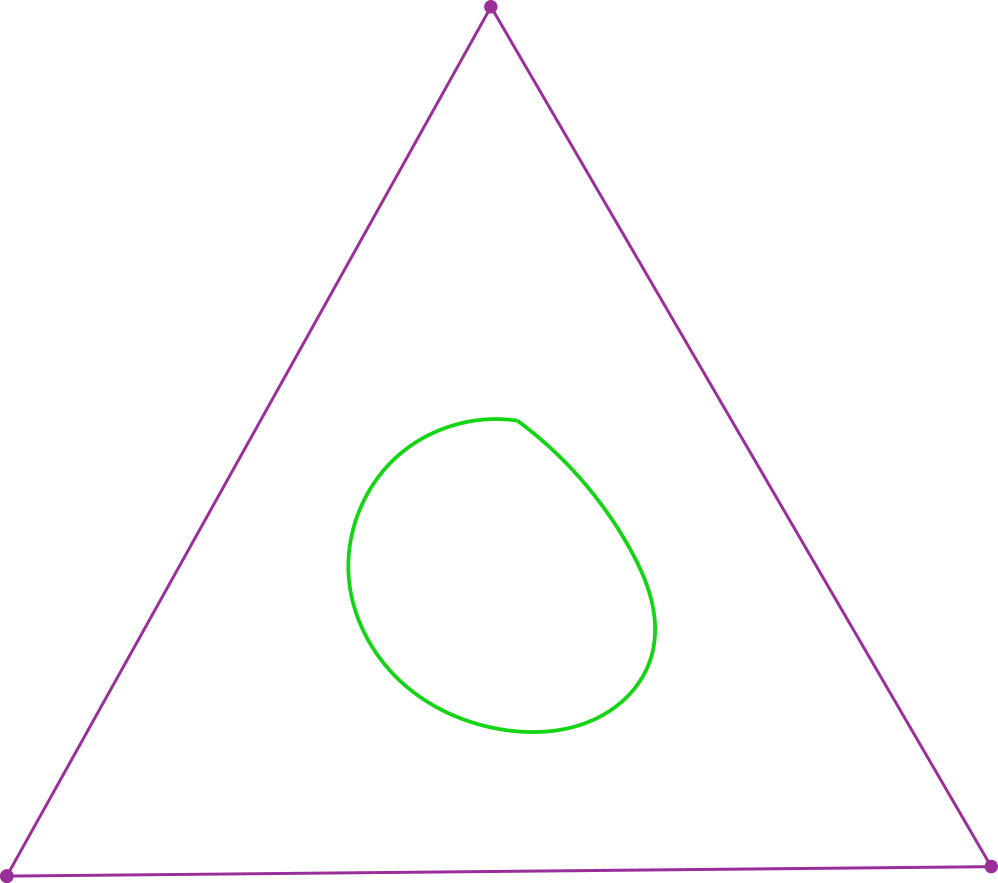
\includegraphics[width=0.5\textwidth]{im1-1}
	\caption{Tres luces iluminan un conjunto convexo y compacto en el Plano.
	\label{im1-1}}
\end{figure}

En 1987, J. O \'Rourke \cite{aguilar_iluminacion_2013}


\bibliographystyle{apalike}
\bibliography{biblio}


\end{document}

%% libro.tex termina aquí.

